% !TEX root = C:/Users/piyus/knowledge/Project_Specific_Knowledge/public/fm_radio/stages/fm_detector/fm_detector.tex
\documentclass[12pt, letterpaper]{article}

\usepackage{hyperref}
\usepackage{graphicx}
\graphicspath{ {C:/Users/piyus/knowledge/Project_Specific_Knowledge/public/fm_radio/stages/fm_detector/pictures} }

\title{FM Detector Notes}
\author{Piyush Sud}
\date{10/20/2024}
\begin{document}
\maketitle

\pagebreak

\section{High Level Design}

There are a few different types of fm detectors that are commonly used:

\begin{itemize}
    \item Foster-Seeley Discriminator
    \item Ratio Detector
    \item Quadrature Discriminator
\end{itemize}

\noindent Out of all of these, the Quadrature Discriminator seems to be the best for a few reasons:

\begin{itemize}
    \item Has a simple design only requiring a few components.
    \item Does not require an RF transformer, which needs to be weakly coupled in the case of the Foster-Seeley Discriminator - cannot easily find one off of digikey/mouser.
    \item Works with low input levels and has good linearity.
\end{itemize}

\section{Principle of Operation}

\begin{figure}[h]
    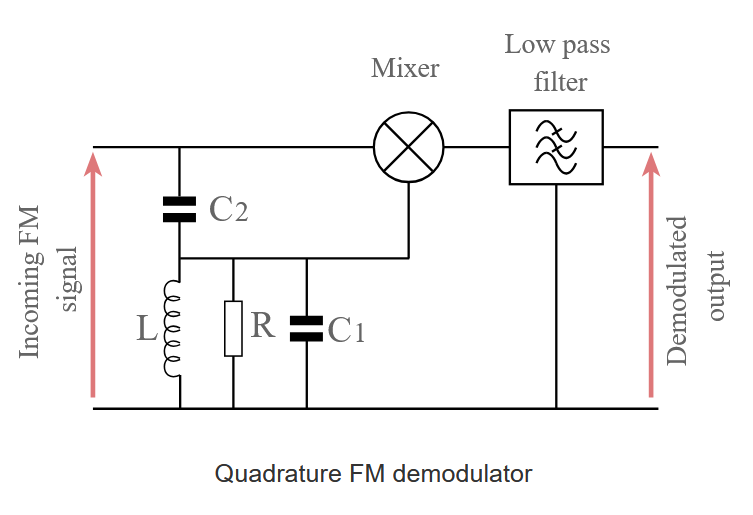
\includegraphics[width=\textwidth]{fm_discriminator}
\end{figure}

The original signal is 

\[Acos(wt)\] 

The signal after C2 is shifted by 90 degrees due to the capacitor, and additionally shifted by \(\phi\) due to the difference between the resonant frequency of the tank circuit and the incoming FM signal. Therefore the signal after C2 is 

\[Acos(wt + \frac{\pi}{2} + \phi)\] 

Multiplying these two together gives 

\[Acos(wt) * Acos(wt + \frac{\pi}{2} + \phi)\] 

By the identity \(cos(a)cos(b) = \frac{1}{2}[cos(a-b) + cos (a+b)] \),

\[= \frac{A^2}{2}cos(-\pi/2 - \phi) + cos(2wt + \frac{\pi}{2} + \phi)\] 

Noting that \(cos(-\pi/2 - \phi) = sin(\phi)\), 

\[= \frac{A^2}{2}sin(\phi) + cos(2wt + \frac{\pi}{2} + \phi)\] 

The higher frequency cosine component can be filtered out, leaving a function whose amplitude is proportional to the phase, which in turn is proportional to \(sin(\phi)\). For small values of \(\phi\), this is approximately equal to \(\phi\).



\section{Detailed Design}

\begin{itemize}
    \item For the tank circuit, the self resonant frequency is given by \( \frac{1}{2\pi \sqrt{RC}}\). If we choose L = 0.1 uH, then for a resonant frequency of 10.7 MHz, this gives us 2.21 nF. 
    \item For the 90 degree phase shift cap, we can use a small 10 pF cap. 
    \item Since the inductor and capacitor values are not exact, the resonant frequency of the tank circuit will not be exactly 10.7 MHz. This will result in a phase error \(\alpha\). We can AC couple the output to solve this issue.
    \item \[ out = \frac{A^2}{2}sin(\phi + \alpha) \]
    \item We need a mixer that can mix down to very low frequencies, since the mono baseband is typically 50 Hz to 15 kHz. We can use the same LT5600 that we used earlier for the IF, since according to \url{https://ez.analog.com/rf/f/q-a/165857/lt5560-low-frequency-performance}, the output goes down to DC.
    \item We can use an op-amp at the output and pullup resistors since transformers are impractical for DIFF to SE conversion at low frequencies, since the size of transformers is inversely proportional to their frequency for a given power transfer.
    \begin{figure}[h]
        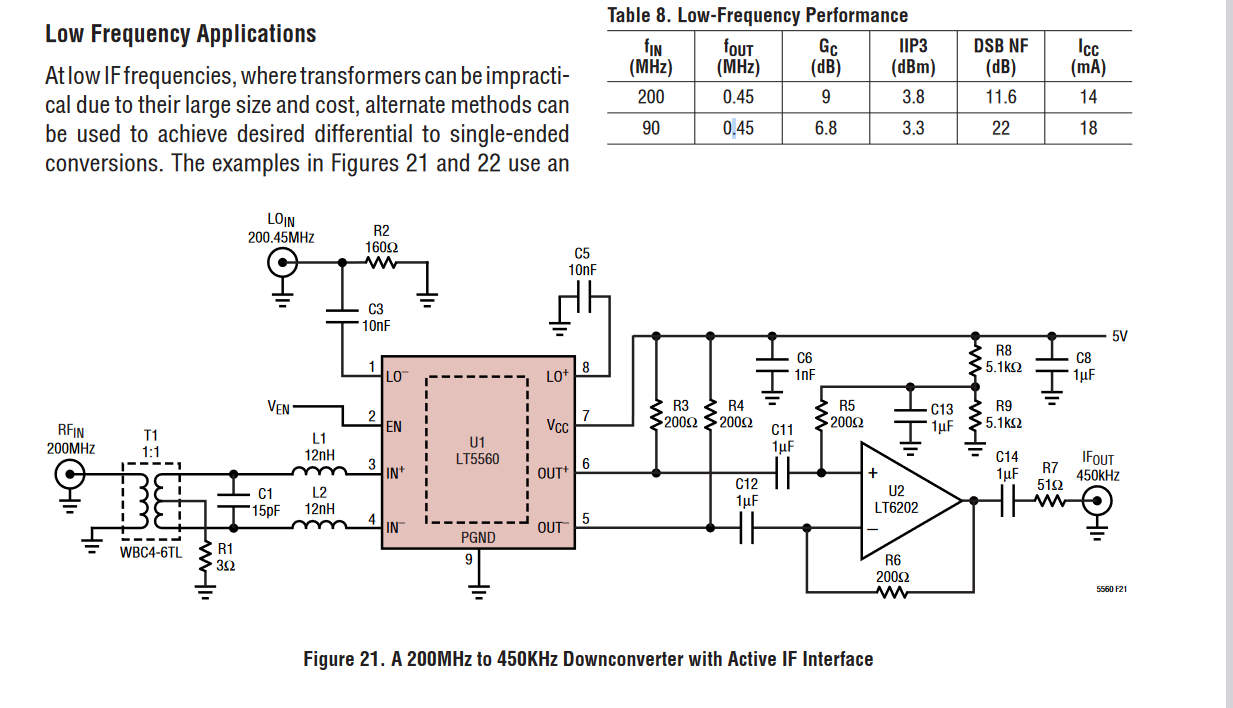
\includegraphics[width=\textwidth]{low_frequency_output}
    \end{figure}
\end{itemize}


\section{Simulations}
 
Here is a simulation of the tank circuit in the discriminator:



\begin{figure}[h]
    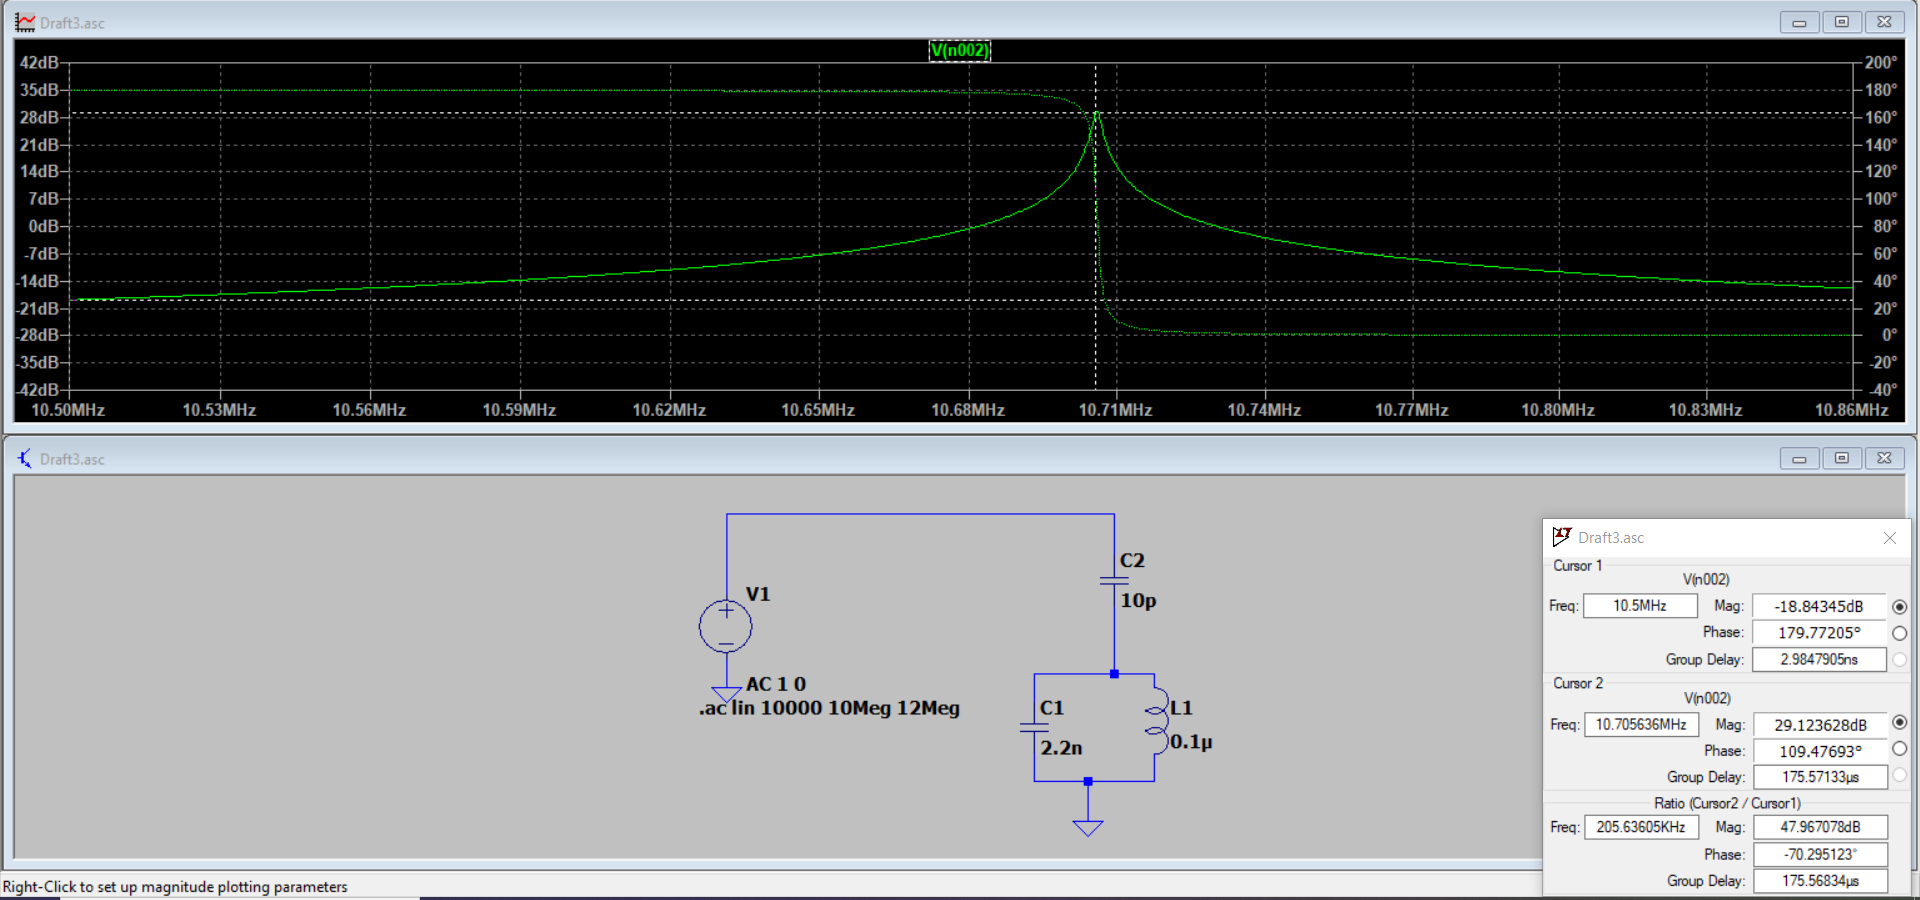
\includegraphics[width=\textwidth]{tank_circuit}
\end{figure}


\end{document}